\section{Experimentos e resultados}\label{sec:resultados}

Cada experimento \'e um script \texttt{matlab/experimentos/expNN\_*.m} que grava tabelas em \arq{resultados/} (CSV) e figuras em \arq{relatorio/figs/}. Esta se\c{c}\~ao resume o que cada um
mede e conclui.

\subsection{Vis\~ao geral}

\begin{center}\small
\begin{tabularx}{\textwidth}{@{}l>{\raggedright\arraybackslash}X>{\raggedright\arraybackslash}Xc@{}}
\toprule
Exp. & O que mede & Resultado principal & Cap. \\ \midrule
E1 & Valida\c{c}\~ao do painel e identificabilidade & Erro de $V_{oc}$ 0,03\,\%; $\gamma_P$ $-0{,}363$ contra $-0{,}4$\,\%/K; efici\^encia em 200\,W/m$^2$ entre 93,1 e 94,8\,\% & \ref{sec:extracao} \\
E2 & Curvas I-V e P-V sob sombra & At\'e 3 picos; o global pode estar em qualquer um & \ref{sec:sombra} \\
E3 & Chaveado contra m\'edio & Concordam em CCM; separam-se em DCM & \ref{sec:conversor} \\
E4 & Bode, margens e degrau do PI & $f_c=56{,}6$\,Hz, MG m\'inima 6,2\,dB, $t_s=20{,}2$\,ms, $\Ta=31$\,ms & \ref{sec:controle} \\
E5 & MPPT est\'atico com sombra & P\&O/InC chegam a 42\,\%; PSO $\ge99{,}99$\,\% & \ref{sec:mppt} \\
E6 & MPPT na EN 50530 & P\&O 99,9\,\%, InC 99,6\,\%, PSO 98,6\,\% & \ref{sec:e6} \\
E6b & Trecho da EN 50530 no modelo din\^amico & Din\^amico e quase-est\'atico concordam & \ref{sec:e6b} \\
E7 & Dia real com sombras e abla\c{c}\~ao & PSO 98,7\,\%; t\'ermico pesa 9\,\%, perdas pesam 11\,\% & \ref{sec:e7} \\
E8 & Modelo anterior contra completo & O anterior superestima a energia em 21,9\,\% & \ref{sec:e8} \\
\bottomrule
\end{tabularx}
\end{center}

\subsection{E6: MPPT na EN 50530 (sem sombra)}\label{sec:e6}

O perfil de cerca de 7\,h \'e simulado no quase-est\'atico, com $T=25\,^\circ$C fixa e or\'aculo a cada 1\,s. A efici\^encia \'e $\eta=E/E_g$, com $E_g=352{,}95$\,Wh dispon\'iveis. O passo $\delta$ do P\&O e
do InC \'e o compromisso cl\'assico: $\delta$ grande segue rampas r\'apidas mas oscila mais em torno do MPP; $\delta$ pequeno oscila pouco mas fica para tr\'as. Por isso varreu-se $\delta=0{,}5$; $1$ e
$2$\,\% de $V_{oc}$ ($\varepsilon$ do InC \'e reescalado junto).

\begin{resultado}
\small\centering
\begin{tabular}{@{}llccc@{}}
\toprule
Algoritmo & $\delta$ [\% $V_{oc}$] & $\eta$ & Energia na bateria [Wh] & Rein\'icios \\ \midrule
P\&O & 0,5 & 99,92\,\% & 323,85 & --- \\
P\&O & 1 & 99,90\,\% & 323,77 & --- \\
P\&O & 2 & 99,62\,\% & 322,92 & --- \\
InC & 0,5 & 98,79\,\% & 319,93 & --- \\
InC & 1 & 99,16\,\% & 321,17 & --- \\
InC & 2 & 99,58\,\% & 322,64 & --- \\
PSO & --- & 98,62\,\% & 319,67 & 2182 \\
\bottomrule
\end{tabular}
\end{resultado}

\textbf{Como ler.} Sem sombra, P\&O e InC t\^em de 99,6\,\% a 99,9\,\% e o PSO \'e 1,3 ponto pior. O motivo: o PSO reinicia a busca a cada rampa (2182 rein\'icios no perfil) e, a cada busca, passa v\'arios per\'iodos avaliando
part\'iculas longe do pico. Quando a luz s\'o varia de forma uniforme n\~ao h\'a pico global escondido, e esse custo n\~ao compensa. O conversor fica em DCM em cerca de 30\,\% do tempo, por causa das irradi\^ancias baixas do perfil (10 a 100\,W/m$^2$).

\subsection{E6b: confer\^encia no modelo din\^amico}\label{sec:e6b}

Um trecho curto da sequ\^encia B.3 ($G$ de 300 a 1000\,W/m$^2$, 50\,W/m$^2$/s, 2 trap\'ezios, 106\,s) roda tamb\'em na \texttt{sim\_dinamica}, com a espera inicial encurtada para 10\,s:

\begin{resultado}
\small\centering
\begin{tabular}{@{}lcc@{}}
\toprule
Algoritmo & $\eta$ din\^amico & $\eta$ quase-est\'atico \\ \midrule
P\&O & 99,88\,\% & 99,88\,\% \\
InC & 99,49\,\% & 99,49\,\% \\
PSO & 97,79\,\% & 97,62\,\% \\
\bottomrule
\end{tabular}
\end{resultado}

Os dois modelos concordam em P\&O e InC, e para o PSO o quase-est\'atico fica 0,2 ponto abaixo, no sentido conservador do Cap\'itulo~\ref{sec:sim}. Os ``dentes'' do PSO na figura s\~ao as buscas.

\begin{figure}[htbp]
\centering
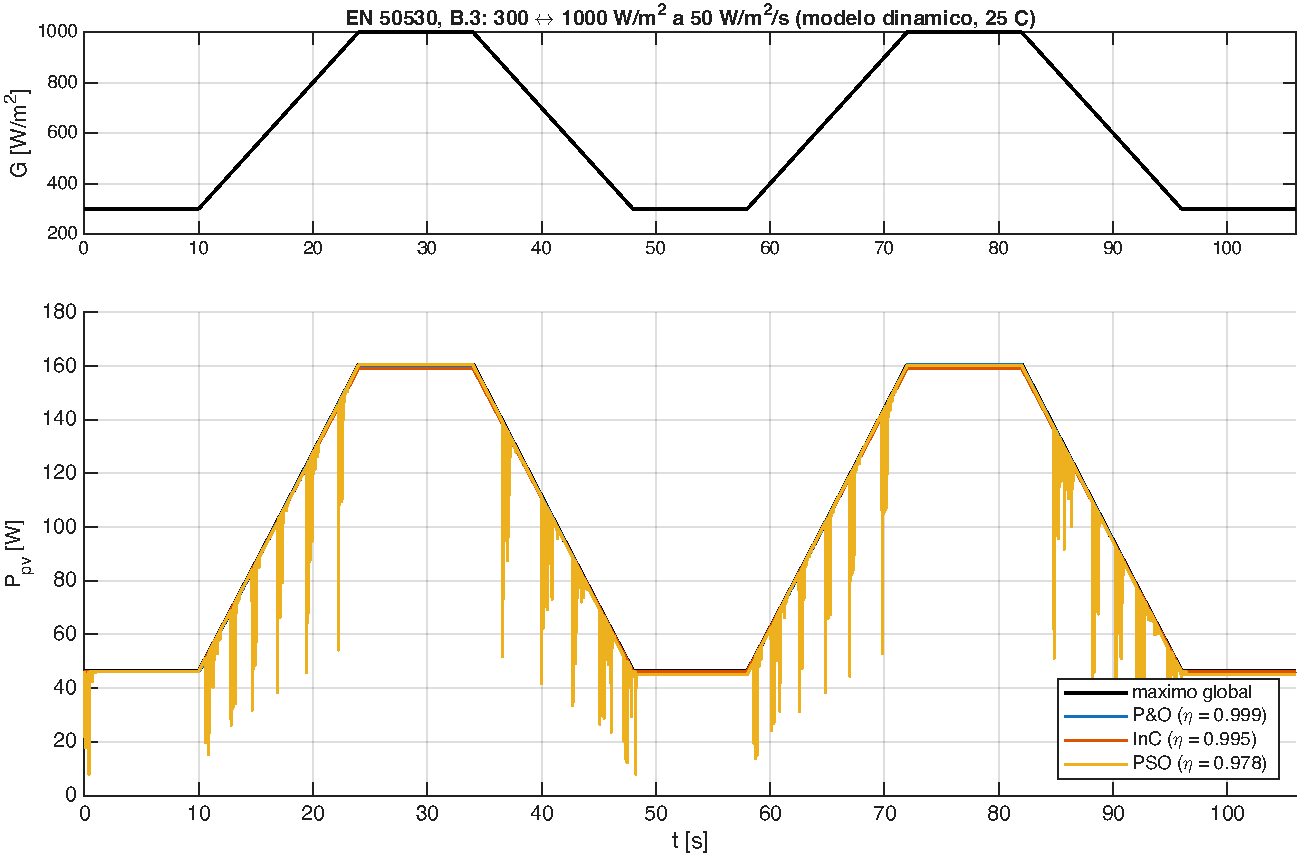
\includegraphics[width=0.95\linewidth]{e6_dinamico.pdf}
\caption{E6b. Como cada algoritmo segue as rampas no modelo din\^amico.}
\label{fig:e6b}
\end{figure}

\subsection{E7: dia em Florian\'opolis com sombras e abla\c{c}\~ao}\label{sec:e7}

O dia 26/01/2020 com os eventos sint\'eticos, no modelo completo, com 3 algoritmos $\times$ 3 variantes (completo, sem t\'ermico, sem perdas) = 9 rodadas de 9 a 23\,min de CPU.

\begin{resultado}
\small\centering
\begin{tabular}{@{}llcccc@{}}
\toprule
Variante & Algoritmo & $E_{pv}$ [Wh] & $E_{bat}$ [Wh] & $\eta$ & $\Delta E_{bat}$ \\ \midrule
Completo & P\&O & 1018,5 & 913,4 & 95,7\,\% & --- \\
Completo & InC & 997,6 & 896,5 & 93,8\,\% & --- \\
Completo & PSO & 1050,8 & \textbf{941,7} & \textbf{98,7\,\%} & --- \\
\midrule
Sem t\'ermico (25\,$^\circ$C) & P\&O & 1108,8 & 993,7 & 95,6\,\% & $+8{,}8$\,\% \\
Sem t\'ermico (25\,$^\circ$C) & InC & 1091,2 & 976,8 & 94,1\,\% & $+9{,}0$\,\% \\
Sem t\'ermico (25\,$^\circ$C) & PSO & 1143,7 & 1020,8 & 98,6\,\% & $+8{,}4$\,\% \\
\midrule
Sem perdas & P\&O & 1018,5 & 1018,5 & 95,7\,\% & $+11{,}5$\,\% \\
Sem perdas & InC & 997,6 & 997,6 & 93,8\,\% & $+11{,}3$\,\% \\
Sem perdas & PSO & 1050,8 & 1050,8 & 98,7\,\% & $+11{,}6$\,\% \\
\bottomrule
\end{tabular}
\end{resultado}

\begin{itemize}
\item \textbf{O PSO ganha na sombra.} Na sombra de poste (14:00 a 15:00), P\&O e InC ficam no pico de alta tens\~ao, com cerca de metade da pot\^encia dispon\'ivel; o PSO reinicia, acha o global e o segue. A energia n\~ao captada, de $\sim$1064\,Wh
 dispon\'iveis, \'e de 13,8\,Wh para o PSO (1,3\,\%), 45,7\,Wh para o P\&O (4,3\,\%) e 66,2\,Wh para o InC (6,2\,\%).
\item \textbf{Na bateria}, o PSO entrega 28,3\,Wh (3,1\,\%) a mais que o P\&O e 45,2\,Wh (5,0\,\%) a mais que o InC.
\item \textbf{O aquecimento pesa 9\,\%.} O m\'odulo chega a 55,6--55,7\,$^\circ$C; ignor\'a-lo aumenta a energia dispon\'ivel em 9,0\,\% e a da bateria em 8,4 a 9,0\,\%.
\item \textbf{As perdas do conversor pesam 11\,\%.} Ignor\'a-las aumenta a energia na bateria em 11,3 a 11,6\,\%; a efici\^encia m\'edia do conversor no dia \'e de 89,6 a 89,9\,\%; o conversor fica em DCM em $\sim$13\,\% dos per\'iodos.
\item \textbf{Os dois efeitos s\~ao maiores que a diferen\c{c}a entre o melhor e o pior algoritmo} (5,0\,\%) e n\~ao mudam o ordenamento: um modelo isot\'ermico ou sem perdas erra a energia mais do que a escolha do algoritmo.
\item O PSO reiniciou 104 vezes no dia. Os eventos de sombra reduzem a energia dispon\'ivel de cerca de 1138\,Wh (o mesmo dia sem eventos) para 1064\,Wh.
\end{itemize}

\begin{figure}[htbp]
\centering
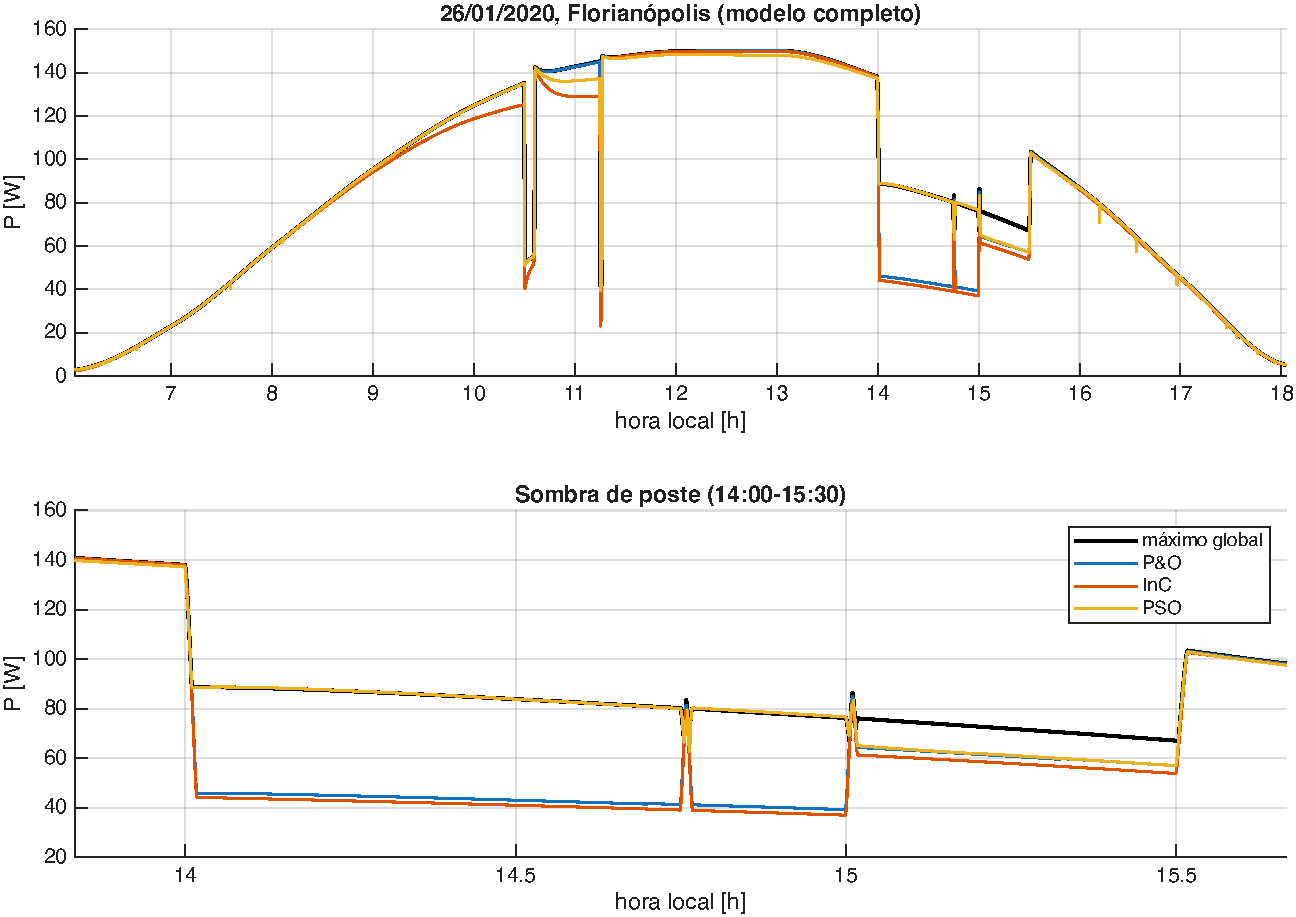
\includegraphics[width=0.95\linewidth]{e7_dia.pdf}
\caption{E7. Pot\^encia ao longo do dia (modelo completo). Preto: m\'aximo global (or\'aculo); demais: pot\^encia extra\'ida por P\&O, InC e PSO. Embaixo, o detalhe da sombra de poste.}
\label{fig:e7}
\end{figure}

\subsubsection{Tr\^es limita\c{c}\~oes que s\'o o dia real revela (D17)}

Ficaram documentadas como resultado, sem alterar os algoritmos (corrigi-las exigiria rodar E6 e E7 de novo, horas de CPU):
\begin{enumerate}
\item \textbf{O PSO n\~ao acompanha a deriva t\'ermica.} Depois de convergir ele fica parado no $g_{best}$. Quando o m\'odulo esquenta de 43 para 53\,$^\circ$C depois da nuvem das 10:30, o $V_{mp}$ cai, mas o PSO s\'o reinicia se a pot\^encia mudar mais de 10\,\%: fica 3 a 4\,\% abaixo do m\'aximo.
\item \textbf{O InC ``congela''.} S\'o sai do lugar se $\Delta I>0{,}2\,\%\,I_{sc}$ por amostra ($\sim$18\,mA); varia\c{c}\~oes lentas de luz n\~ao chegam a isso.
\item \textbf{O PSO erra o pico global com sombra fraca e m\'odulo quente.} Com $[1\ 1\ 0{,}5]\cdot656$\,W/m$^2$ a 44\,$^\circ$C, as part\'iculas iniciais erram o pico global (11,6\,V) e o enxame converge no local (18,9\,V).
\end{enumerate}

\subsection{E8: o trabalho anterior contra o modelo completo}\label{sec:e8}

O mesmo dia, sem os eventos de sombra, com P\&O nos dois casos e o mesmo PI. O modelo ``anterior'' usa 1 diodo, conversor ideal e c\'elulas a 25\,$^\circ$C; o ``completo'', 2 diodos, perdas e t\'ermico.

\begin{resultado}
\small\centering
\begin{tabular}{@{}lccc@{}}
\toprule
Modelo & $E_{pv}$ [Wh] & $E_{bat}$ [Wh] & $T_{m\acute ax}$ [$^\circ$C] \\ \midrule
Anterior (1 diodo, ideal, 25\,$^\circ$C) & 1238,4 & 1238,4 & 25,0 \\
Completo (2 diodos, perdas, t\'ermico) & 1137,2 & 1015,8 & 55,6 \\
\bottomrule
\end{tabular}
\end{resultado}

O anterior \textbf{superestima a energia na bateria em 21,9\,\%} ($1238{,}4/1015{,}8=1{,}219$). A diferen\c{c}a se decomp\~oe de forma multiplicativa: as perdas do conversor respondem por
$1137{,}2/1015{,}8=1{,}120$ ($+12$\,\%); o resto, $1238{,}4/1137{,}2=1{,}089$ ($+9$\,\%), re\'une a temperatura e a troca de 2 para 1 diodo. Como s\'o a temperatura j\'a aumenta a energia
dispon\'ivel em 9,0\,\% no E7, a contribui\c{c}\~ao do modelo de 1 diodo \'e praticamente nula, coerente com o E1 (os dois modelos s\~ao ajustados aos mesmos pontos e diferem pouco perto de STC, onde est\'a quase toda a energia de um dia de ver\~ao).
\textbf{O erro n\~ao estava no n\'umero de diodos, mas no que ficou fora do modelo.}

\begin{atencao}[: ressalva]
O E8 \'e uma \emph{reconstru\c{c}\~ao}: o modelo ``anterior'' usa o ajuste de 1 diodo bem posto deste trabalho, para isolar o efeito das simplifica\c{c}\~oes. A extra\c{c}\~ao original do trabalho anterior dava $\sim$121\,W com o MPP perto de 15\,V, contra 160\,W
em 19,6\,V aqui. Esse erro de par\^ametros se somaria \`as simplifica\c{c}\~oes e n\~ao est\'a nos 21,9\,\%.
\end{atencao}
